\section{OpenMP}

OpenMP es una interfaz de programación paralela para \textbf{arquitecturas multiprocesador de memoria compartida}, diseñado para proporcionar una interfaz portable, escalable y de alto nivel que permita explotar el paralelismo en CPUs multinúcleo sin recurrir a APIs de hilos de bajo nivel. Su diseño se basa en directivas de compilador, rutinas de biblioteca y variables de entorno. Sigue el modelo de ejecución \textit{fork–join}, donde un hilo maestro crea y sincroniza equipos de hilos que ejecutan regiones paralelas \cite{Jin2024}.

\begin{figure}[H]
	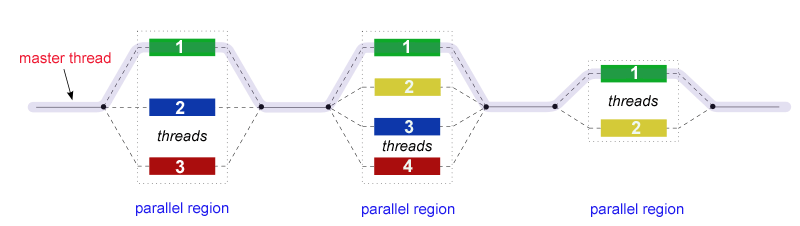
\includegraphics[width=\linewidth]{imagenes/fork-join.png}
	\caption{Modelo \textit{fork-join} \cite{Lawrence2019}}
	\label{fig:fork-join}
\end{figure}

Surge en 1997, cuando Intel impulsa la creación del OpenMP Architecture Review Board (ARB), un consorcio formado por fabricantes de hardware y software (Intel, IBM, AMD, HP, Nvidia, Oracle, entre otros) con el objetivo de definir un estándar común para paralelismo en memoria compartida. La última versión de OpenMP, la 6.0, data de 2024.

OpenMP aprovecha el paralelismo mediante \textit{multithreading}. El funcionamiento es relativamente simple, el programa comienza con un comportamiento secuencial y un hilo maestro. Cuando este hilo se encuentra una región paralela específica con \texttt{\#pragma omp parallel}, se crea un equipo de hilos \cite{ARB2024}. Los hilos ejecutan el bloque paralelo de forma concurrente, y al finalizar, los hilos se unen y el control vuelve al maestro.

Podemos identificar varios elementos principales, el primero de los cuales sería las directivas de compilador, como \texttt{\#pragma omp parallel}, \texttt{\#pragma omp for}, o \texttt{\#pragma omp single}, y sus cláusulas como \texttt{schedule}, \texttt{shared}, o \texttt{default}. Otros elementos importantes son las funciones de biblioteca, como \texttt{omp\_set\_num\_threads()} o \texttt{omp\_get\_wtime()}, y las variables de entorno, como \texttt{OMP\_NUM\_THREADS}, \texttt{OMP\_SCHEDULE}, o \texttt{OMP\_DYNAMIC}. \cite{ARB2024} 

Como hemos comentado, OpenMP opera sobre un modelo de memoria compartida en la que todos los hilos ven el mismo espacio de direcciones de memoria, en el que las variables pueden ser visibles por todos los hilos ($shared$), o cada hilo tiene su propia copia de una variable ($private$). Este modelo evita la necesidad de comunicación explícita entre procesos (como en MPI)\cite{Jin2024}, simplificando el desarrollo. 

\section{CUDA}

\textbf{CUDA}, siglas de \textit{Compute Unified Device Architecture} es una plataforma de computación paralela y un conjunto de APIs desarrollado por NVIDIA para ejecutar código general en sus GPUs. Incluye, entre otros, un modelo de programación a partir de C y C++; herramientas de compilación que generan código tanto para CPU como para GPU; un entorno de ejecución y una API para gestionar memoria, lanzamientos de kernels, streams; y librerías construidas sobre el propio modelo \cite{Kirk2010}. La idea principal es permitir que el programador trate a la GPU como un dispositivo de \textbf{cómputo masivamente paralelo}.

A modo de referencia, los primeros trabajos en los que se utiliza una GPU para cómputo general aparecen a principios de los 2000, en 2004 se crea internamente CUDA, y se lanza oficialmente en 2007. Desde entonces, la evolución de CUDA ha ido ligada a la evolución propia de las GPUs de NVIDIA, manteniendo el modelo de ejecución \textbf{SIMT}\textit{(Single Instruction, Multiple Threads)} y añadiendo unidades especializadas como \textit{Tensor Cores}, \textit{Ray Trancing Cores}, o el mecanismo del \textit{Transformer Engine} \cite{NVIDIA2026}.

CUDA implementa un modelo SIMT, en el cual el programador define una función denominada kernel que describe el código de un hilo, que se lanza desde la GPU y se ejecuta de forma concurrente en la GPU usando múltiples hilos. Los hilos se agrupan en bloques, que son arrays tridimensionales de hilos; y los bloques a su vez se agrupan como una grid, array tridimensional de bloques. Cada bloque se ejecuta en un \textit{Streaming Multiprocessor}, dentro del cual los hilos se agrupan en \textbf{warps de 32 hilos} que se ejecutan físicamente en paralelo utilizando cores del multiprocesador. \cite{Kirk2010} El warp de hilos es, por tanto, la unidad de ejecución con la que trabajamos.

\textbf{\Huge AÑADIR FIGURA DIAPOSITIVAS PROFESOR}

Cuando se programa con CUDA se ha de tener en mente que se puede acceder a varias \textbf{memorias diferentes}, cada una con su propia latencia y ancho de banda, y entre ellas nos encontramos a los \textbf{registros}, que son la memoria de los hilos individuales, y la más rápida de todas; pasando por la \textbf{memoria compartida} (\texttt{\_\_shared\_\_}), que usan los bloques; la \textbf{memoria de constantes} (\texttt{\_\_constant\_\_}), que es de solo lectura, y va cacheada; y la \textbf{memoria global}, que se aloja en la VRAM de la GPU, que es la que se utiliza para almacenar grandes estructuras de datos. \cite{Farber2011}

\begin{figure}[H]
	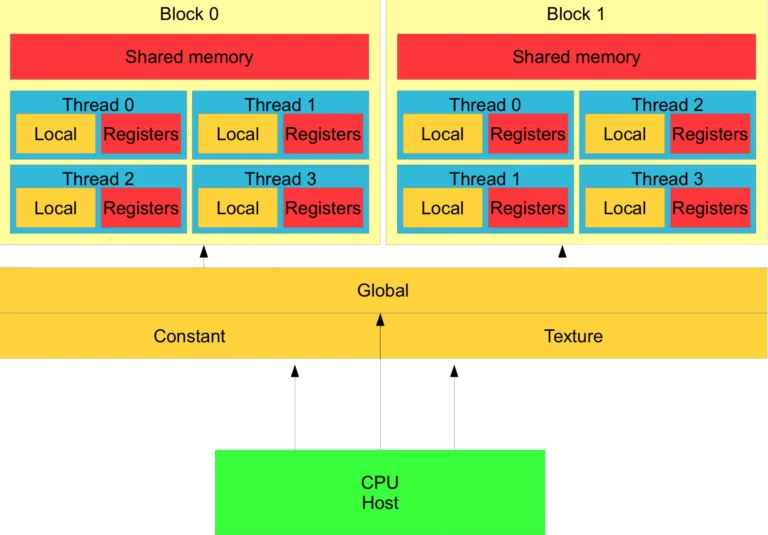
\includegraphics[width=\linewidth]{imagenes/CUDA-Memory-Hierarchy.png}
	\caption{Jerarquía de memorias en CUDA \cite{Beard2020} }
	\label{fig:CUDA-Memory-Hierarchy}
\end{figure}

El rendimiento de la memoria dependerá del buen hacer del programador, que será el encargado de buscar la coalescencia en los accesos a memoria global, del uso de  para reutilizar datos, de que evite la divergencia de los warps, y de que se encargue de controlar los warps activos. 

La \textbf{máxima coalescencia} ocurre cuando los 32 hilos de un warp acceden a direcciones de memoria que caen dentro del mínimo número de segmentos continuos necesarios para almacenar dichos datos \cite{Kirk2010}. Esto permite que la GPU atienda todos esos accesos el mínimo número de trabsacciones, lo cual implica la mayor eficiencia en el kernel al acceder a esos datos en memoria VRAM. 

Por otro lado, la \textbf{divergencia de warps} ocurre cuando los hilos de un mismo warp toman caminos distintos en una rama condicional. Como el warp ejecuta las instrucciones en modo SIMT, si los hilos divergen, el hardware debe serializar las rutas \cite{Farber2011}. Esto quiere decir que si los hilos se encuentran frente a un bloque if/else, lo que va a pasar es que el bloque if será ejecutado por los hilos que cumplan la condición, y el resto de hilos se quedarán en stand-by. A continuación, el resto de los hilos ejecutará el bloque else mientras los primeros se quedan esperando, y luego se combinarán los resultados.

Hay un matiz importante a tener en cuenta a la hora de describir la implementación CUDA, y es que lo que veremos a continuación serán funciones kernels, y no métodos de clase como vimos en el capítulo anterior. Una forma de verlo es que tendremos clases (como \texttt{Metodo}), y éstas tendrán sus funciones miembro que accederemos de forma normal con un objeto de la clase. Por otro lado tendremos las funciones kernel, que podrán ser llamados o no desde los métodos de las clases, y será donde ocurra el paralelismo de CUDA.

Aunque tengamos los kernel implementados en los archivos \texttt{.cu} de las clases, formalmente no son parte de ellas, son métodos globales que pueden ser llamados desde cualquier parte del código.

Como antes mencionamos, los kernel CUDA funcionan con \textbf{grids, bloques, y hebras}, y estos elementos interaccionan entre sí. Cuando llamamos a un kernel se crea una grid, que no es más que un conjunto de bloques con un tamaño predeterminado. Esta grid podrá tener una, dos, o tres dimensiones, y en cualquiera de los casos contendrá un número determinado de bloques. Estos bloques a su vez también tendrán de una a tres dimensiones y contendrán a las hebras, que serán con las que nosotros trabajaremos, indicando a cada hebra qué hacer dentro del kernel.

Aquí podemos ver un ejemplo ilustrativo en el que un kernel particular es llamado y crea una grid bidimensional de bloques, y a su vez los bloques por dentro son tridimensionales.

\begin{figure}[H]
	\centering
	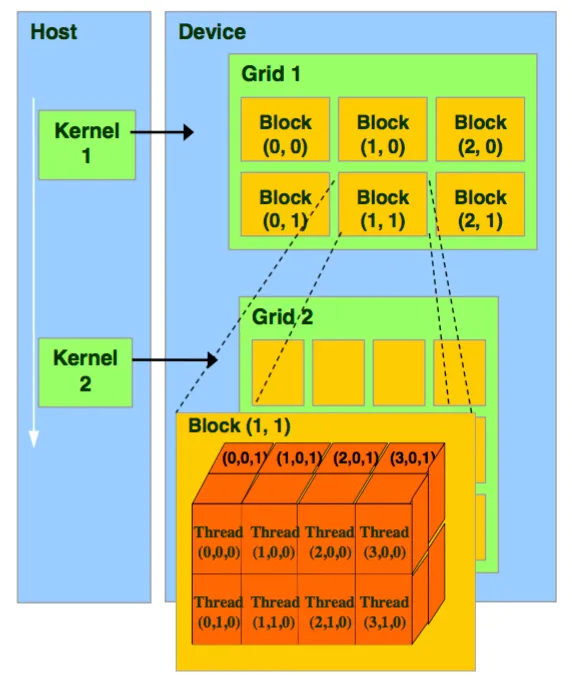
\includegraphics[width=0.65\linewidth]{imagenes/CUDA-blocks-grids.png}
	\caption{Grids y bloques CUDA \cite{Casas2024}}
	\label{fig:CUDA-blocks-grids}
\end{figure}

Como primer ejemplo para ilustrar el modelo, podemos tomar una función auxiliar de la clase \texttt{Metodo} como la que ya vimos implementada en OpenMP (algoritmo \ref{alg:VectorCopia-OMP}), y transformarla al paradigma de programación de CUDA. 

\begin{algorithm}[H]
	\begin{algorithmic}
		\State $ i \gets \text{blockDim.x} \cdot \text{blockIdx.x + threadIdx.x} $
		\If{ $ i < N $ }
		\State $ Y[i] \gets X[i]$
		\EndIf
	\end{algorithmic}
	\caption{Kernel de vectorCopia}
	\label{alg:Vector-Copia-CUDA}
\end{algorithm}

Por un lado, como podemos ver en la primera línea, se calcula un valor $i$ que es igual a una multiplicación y una suma. Identificando a esos 3 elementos tenemos primero a \texttt{blockDim.x}, que es un valor igual al tamaño de la dimensión X del bloque al que pertenezca cada thread particular. Luego, \texttt{blockIdx.x} designa al bloque individual que contenga cada thread que ejecute el kernel, y de igual manera \texttt{threadIdx.x} será el identificador individual de cada thread dentro de su bloque. Combinando los 3 generamos un identificador único para cada uno de los threads que genere el todo el grid.

Por otro lado, se hace la comprobación de que el identificador del thread es menor que el tamaño de los vectores para evitar posibles accesos erróneos a memoria. Esto ha de hacerse ya que, si tenemos un tamaño de problema N, se generará un grid con tantos bloques de tamaño \texttt{blockDim.x} como para que el total de hebras sea siempre mayor o igual a N. Dicho de otra forma, con un tamaño de bloque de 256, y un tamaño de problema de 1000, se generaría una grid con 4 bloques (y por tanto 1024 hebras), y las últimas 24 no trabajarían.